\section{Recorded evidence}
All values in this section are transcribed from frozen native artifacts,
identified in Appendix~\ref{app:artifacts}. This paper build introduces no
new solver experiment or timing measurement. Counts of assignments below
are component correctness controls, not independent hard benchmark instances.

\subsection{Independent small oracles and field coverage}
The original norm compiler records 73,216 complete primary assignments
across eight small $\F_4,\F_8,\F_{16}$ models \ev{E1,E2}.
The bounded-cone transformation records 116,480 complete-assignment checks
in $\F_4,\F_8$ across its seven limits. Seven native complete enumerations
agree on a 28-model fixture \ev{E2}. The changed search driver records
2,048 independent literal-norm assignments and six complete 28-model native
sets, plus cap-one and expired-budget checks \ev{E3}.
These panels vary target signs and include even extensions and zero or
repeated sources. Literal polynomial arithmetic is independent of the
compiler equations; it is not an independent author's replay.

The symmetry preparation records 34,816 literal assignments over eight
small cases \ev{E4}. Six cases restore 28 ordered norm-primary witnesses
from six sorted representatives; two restore 168 from fifteen. Orbit
sizes include one, five, ten, and thirty. All restored sets agree exactly
with the full literal sets. No timing ratio is inferred from these counts.

\begin{table}[tb]
\centering\small
\begin{tabular}{p{0.23\linewidth}p{0.34\linewidth}p{0.33\linewidth}}
\toprule
Component & Recorded field coverage & Established scope\\
\midrule
Binary norm chart and compiler & Tiny binary extensions; one actual
$\F_{2^{83}}$ search fixture & Primary-predicate equivalence and bounded
search diagnostics \ev{E1--E3}\\
Source symmetry & $\F_4,\F_8$, eight cases & Exact norm orbit restoration;
no hard comparator search \ev{E4}\\
Odd supplied-quintic adapter & Eleven odd fields, including all five
NIST prime sizes & Roots and multiplicities of supplied polynomials;
no multivariate coefficient search \ev{E5}\\
\bottomrule
\end{tabular}
\caption{Field coverage is stated per component. It does not certify a
comprehensive all-roots solver across these fields.}
\label{tab:coverage}
\end{table}

The odd adapter first forms $G=\gcd(H,X^q-X)$, where $q=|K|$,
then splits this squarefree product of all distinct field-root factors.
It verifies that the product of returned distinct linear factors is exactly
$G$; exact division in $H$ recovers multiplicities. A bounded splitting
failure returns unresolved. This is classical finite-field factoring,
with a coverage certificate for a supplied polynomial, rather than a new
multivariate algorithm.

The recorded wide test comprises 66 known-answer quintics over eleven
fields: $\F_3$, $\F_5$, $\F_7$, $\F_{11}$, $\F_9$, $\F_{25}$, and the prime fields
of NIST P-192, P-224, P-256, P-384, and P-521 \ev{E5}.
The five prime interval widths are respectively 40, 47, 53, 79, and 106
bits. The adapter also records 3,624 tiny-field controls with independent
Hasse-derivative multiplicities. These tests cover repeated and nonrational
factors. They demonstrate a supplied-polynomial component at large
characteristics; they do not establish a corresponding prime-field norm
search, all scale sizes, or every index-calculus implementation.

\subsection{Actual binary instance and representation profile}
The fixed fixture \ev{E0} uses
\[
 \begin{split}
 K&=\F_2[\theta]/(\theta^{83}+\theta^{45}+\theta^2+\theta+1),\\
 D&=\operatorname{span}_{\F_2}\{1,\theta,\ldots,\theta^{17}\},\\
 E&:\quad Y^2+XY=X^3+1 .
 \end{split}
\]
The full curve identifier is
\texttt{icv1-f2m83-tm6151469093347-debefd74}.
It is a recorded binary fixture, not a named NIST binary-curve preset.
Its original five-source chain contains 339 Boolean variables and 332
equations; the norm chart has 174 primary bits. These dimensions do not
prove equivalence of the two complete solution sets.

\begin{table}[tb]
\centering\small
\begin{tabular}{lrrrr}
\toprule
Support limit & External & XOR rows & Actual internal & Pre-clean estimate\\
\midrule
1 &58,176&44,921&58,176&58,176\\
2 &40,148&26,893&45,427&45,427\\
4 &30,509&17,254&55,395&55,395\\
8 &26,389&13,134&74,121&74,121\\
16&23,754&10,499&106,094&106,094\\
32&22,121&8,866&not loaded&161,033\\
Dense&16,134&2,879&not loaded&910,133\\
\bottomrule
\end{tabular}
\caption{Native cut-aware representation profile \ev{E2}. All arms have
174 primary variables and 39,742 CNF clauses before native XOR cuts.
The last two exceed the preregistered 150,000-coordinate estimate cap.
There is no SAT solve or Gaussian initialization in this profile.}
\label{tab:profile}
\end{table}

\begin{figure}[tb]
\centering
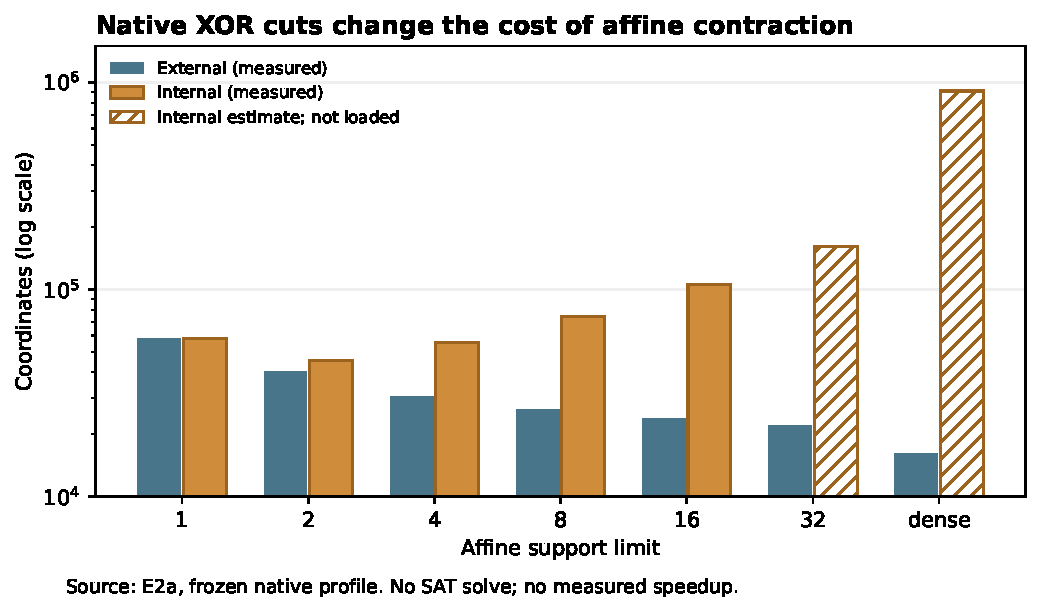
\includegraphics[width=\linewidth]{figures/native_coordinates.pdf}
\caption{Recorded variables for the fixture identified above \ev{E2}.
Measured post-flush internal counts are shown only for loaded arms.
Hatched bars are estimates for capped arms, not measurements. Logarithmic
scale exposes native expansion. Coordinate reductions are not speedups.}
\label{fig:profile}
\end{figure}

Limit two has 21.9\% fewer actual native coordinates than limit one
(Table~\ref{tab:profile}). Dense substitution has the smallest external
count and the largest pre-cleaning internal estimate. This refutes use of
the external variable count alone as the representation-selection criterion.
Limit two was selected after observing this training profile; it is not
a holdout winner.

\subsection{Hard search: a negative bounded result}
The next preregistered worker \ev{E3} asked whether the changed limit-two
representation would produce at least one replayed norm witness or complete
norm exhaustion within its 60-second inner budget. It did neither.
The supervisor records 61.794 seconds cold wall lifetime and 385,368 KiB peak
process RSS. The native inner lifetime is 61.510 seconds, including its
reported overshoot. These are development diagnostics; qualified exclusive
isolation and a matched baseline were not established.

The final verdict is UNKNOWN, with zero verified norm witnesses, null exact
norm count, and null original-system count. One Gaussian matrix was
initialized, peaking at 9,169 rows and 22,491 columns; no row or column
admission cap was rejected. The record includes 7,167 conflicts,
12,065 primary decisions, zero auxiliary decisions, and 28,207,875 Gaussian
row XORs \ev{E3}. The evidence narrows the failure: matrix admission occurred,
but useful search completion did not follow within the budget. It does not
show that a witness is absent.

The worker used one CPU, a 4 GiB per-process address-space cap, a 90-second
outer supervisor, and a 4,096-model output cap. Successful process exit only
means that the diagnostic envelope was serialized. The bounded first-witness
prediction is refuted; the general research objective is still open.
No ratio against an earlier timeout or a Gr\"obner baseline is computed.
